\section{Process for synchronization}
\label{sec:collaboration}
This section describes RAOES's process to synchronize a model with USMs and front-end code in case that these artifacts concurrently evolve.
We assume then use of an integrated development environment (IDE) %used by software architects and programmers 
offering the use-cases defined in Section \ref{subsec:mdrtebackground}. 
%Although, the pattern is presented in a model-code synchronization-oriented way, it is flexibly extensible to any artifacts. 
%For the sake of generality, we postulate that the architect and programmer are actors with starkly opposite development practices.
The process allows concurrent modifications made to the model
and front-end code so that in the end we obtain a full system.
%rather than just architectural design for the former,
%and code implementation for the latter.


We propose two synchronization strategies.
The rationale behind our strategies
is to represent one artifact (model or front-end code) in the language of its corresponding other artifact (front-end code or model).
%These two can then be compared. 
For this, we define the
concept of a \ttt{synchronization artifact}:

\begin{definition}[Synchronization artifact]
	An artifact used to synchronize a model and its corresponding front-end code
	is called a synchronization artifact.
	It is an image of one of the artifacts, either the model or the front-end code.
	In this context, an image $I$ of an artifact $A$ is a copy of $A$ obtained by
	transforming $A$ to $I$. $A$ and $I$ are semantically equivalent but are specified in different languages.
\end{definition}

For example, a synchronization artifact (SA) can be code that was generated from the edited model in batch mode.
In that case, it is code that represents an image of the edited model (being image requires that the model is able to be reconstructed from the code).

Using the concept of SA, two strategies are
proposed: one in which the SA is code,
and the other in which the SA is a model.
The developer can choose to either use these two use-cases of the IDE. 
The choice may be determined by
preferred development practices or the availability of suitable tools (e.g. the programmer
may prefer to synchronize two artifacts, both represented
in the same programming language, since he prefers to
work exclusively with code).

Figure \ref{fig:scenario3} shows the first synchronization
strategy based on using front-end code as SA.
The general steps of the process shown in Figure \ref{fig:scenario3} are described as follows:

\begin{figure}
	\centering
	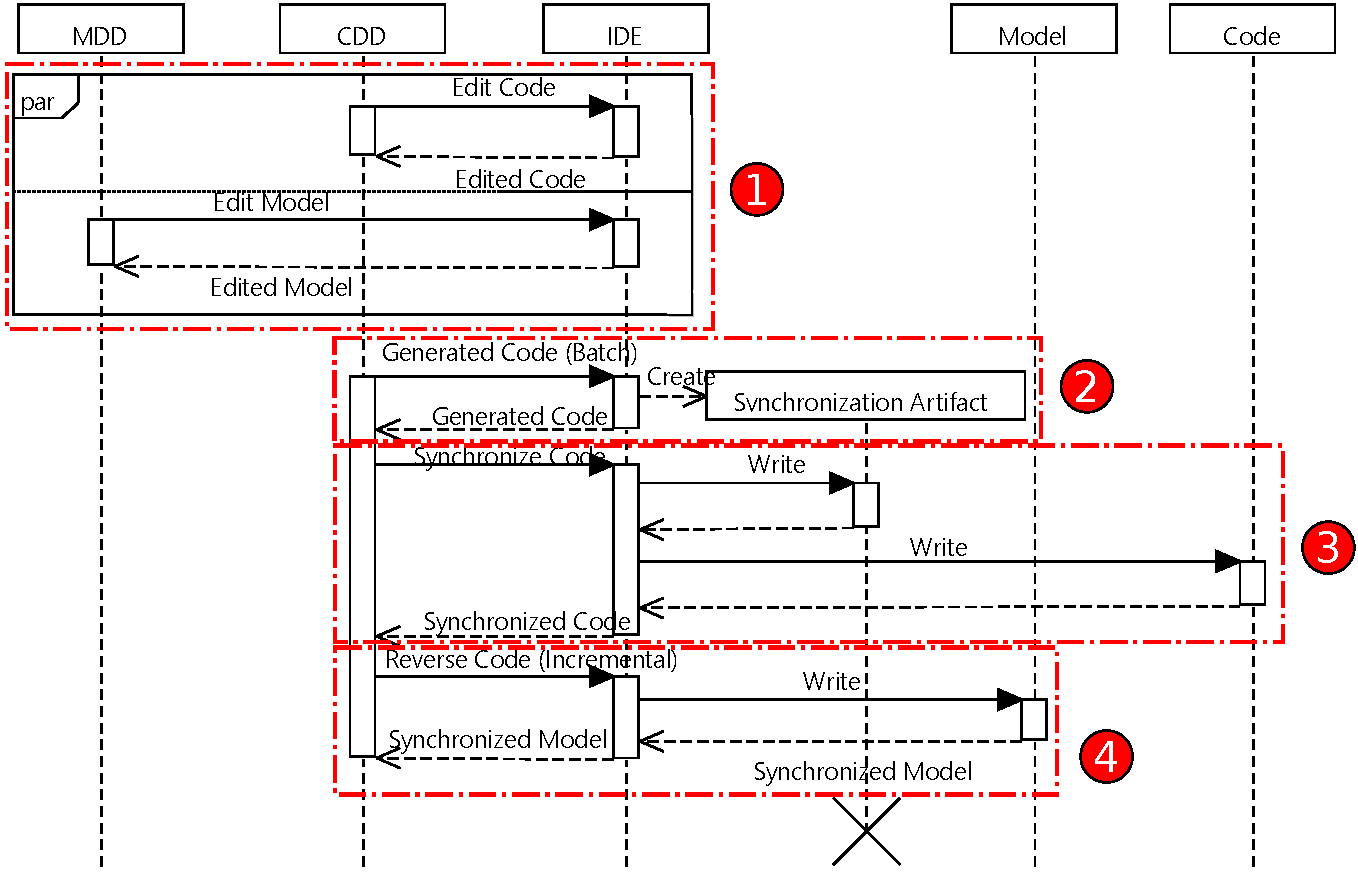
\includegraphics[width = \columnwidth]{figures/scenario3_seq}
	\caption{Synchronization process, in which the model and the code are concurrently edited with code as the SA (CDD = Code-Driven Developer = Programmer, MDD = Model-Driven Developer = Software Architect, Code = C++ front-end code). The API calls for Model and Code are represented generically as "Read" and "Write".}
	\label{fig:scenario3}
\end{figure}

\begin{description}[\footnotesize]
	\item[Step 1] Both the model and code may be edited concurrently.
	%(To simplify Figure \ref{fig:scenario3}, we don't show the Read and Write interactions for this step.)
	%After both artifacts have been edited concurrently, we need to synchronize them.	
	\item[Step 2] First we create an SA from the edited model by generating front-end code in batch mode.
	This SA is code and it is an image of the edited model.	
	
	\item[Step 3] The SA is synchronized with the edited code. Since the SA
	is code itself, this step is done with the \texttt{Synchronize Code} use-case of the IDE.
	
	\item[Step 4] Once SA and edited code are synchronized, the former is reversed incrementally to update the edited model.
\end{description}

The second strategy, based on using the model as the SA,
is the opposite of the first strategy. 
In the second strategy, the SA is
obtained by reversing the edited code in batch mode.
Afterwards the SA is synchronized with the edited model.
Finally, we generate code incrementally from the SA to update the edited code.

%Figure \ref{fig:strategy2} shows the synchronization strategy based on using model as the synchronization artifact.
%This strategy is the opposite of the strategy presented in Figure \ref{fig:strategy1}. Its steps are described as follows:
%
%\begin{center}
%\textbf{\textit{- Steps of synchronization strategy 2 -}}
%\end{center}
%\begin{description}
%	\item[Step 1] The synchronization artifact is obtained by reversing the edited code in batch mode.
%	\item[Step 2] Afterwards the synchronization artifact is synchronized with the edited model.
%	\item[Step 3] Finally, we generate code incrementally from the synchronization artifact to update the edited code.
%\end{description}
%
%\begin{figure}
%\centering
%\includegraphics[width=\columnwidth]{figures/strategy2}
%\caption{Synchronization strategy 2 using model as synchronization artifact}
%\label{fig:strategy2}
%\end{figure}

The actors may even use both strategies, successively, as a kind of hybrid strategy.
This may be useful
when developers want to synchronize some parts of the system using one strategy,
and other parts using the other strategy. %For example, they may choose
%to synchronize method bodies using strategy 1, where the synchronization artifact is code.
%Then strategy 2, in which the synchronization artifact is a model, is used to
%to synchronize architectural elements of the system.

%In reality of collaboration, there are of course conflicts between editions made by developers to their respective baseline artifact.
%Two approaches are proposed to reconcile these conflicts.
%In the first approach, we let the developers explicitly determine which edition should be kept in the synchronization process.
%This is based on the \texttt{Compare and Merge} paradigm proposed by model/code merge tools such as \textbf{EMF Compare} or \textbf{Git}.  
%The second approach extends the semi-automated conflict resolution presented in \cite{Hermann2012}.
%Specifically, our approach records editions made to artifacts (see Section \ref{sec:implementation} for more information about edition listening), decides whether editions are \textit{conflict-free} or not, and automatically bi-directionally merges or interactively shows the developers in-conflict editions.
%For example, if an MDD adds an attribute to a class by using graphical modeling tools and a CDD renames the class.
%Two editions are detected and asserted as conflict-free. The automated merge therefore is used for reconciliation. 

%In the next section we propose an implementation
%of an IDE and the proposed synchronization processes.